\chapter{Transformada de Fourier}

\section{Definiciones}

Aprendimos que la serie de Fourier de $f \in \mathcal{C}[-L/2,L/2]$ está dada por 
\begin{equation}
  f(x) = \sum_{n=-\infty}^{\infty} c_n e^{i \frac{2n\pi}{L}x},  \label{Transformada1}
\end{equation}

donde 
\begin{equation}
  c_n = \frac{1}{L} \int_{-L/2}^{L/2} f(x) e^{-i\frac{2n\pi}{L}x} \,dx, \quad n \in \mathbb{Z}. \label{Transformada2}
\end{equation}

Una consecuencia inmediata de la expansión en serie de Fourier es que la función $f(x)$ representada por la serie resulta periódica, con período $L$. Por lo tanto, decimos que la serie de Fourier permite expandir funciones periódicas. Sin embargo, no todas las funciones son periódicas. Necesitamos, entonces, algún modo de expandir, en una base ortonormal, funciones no periódicas. 

Podemos decir que el conjunto de coeficientes $\{c_n\}$ también definen a $f(x)$. Este conjunto de números $c_n$ puede ser entendido como una función en la variable $n$, escrita como $c(n)$, definida para un conjunto \underline{discreto} de valores de la variable independiente (en lugar de un intervalo continuo).  La función $c(n)$ es a menudo llamada el \textbf{espectro de Fourier} de $f(x)$ y puede ser graficado, asumiendo $c(n)$ real, como sigue.

\vspace{-0.5cm}
\begin{figure}[H]
    \centering
    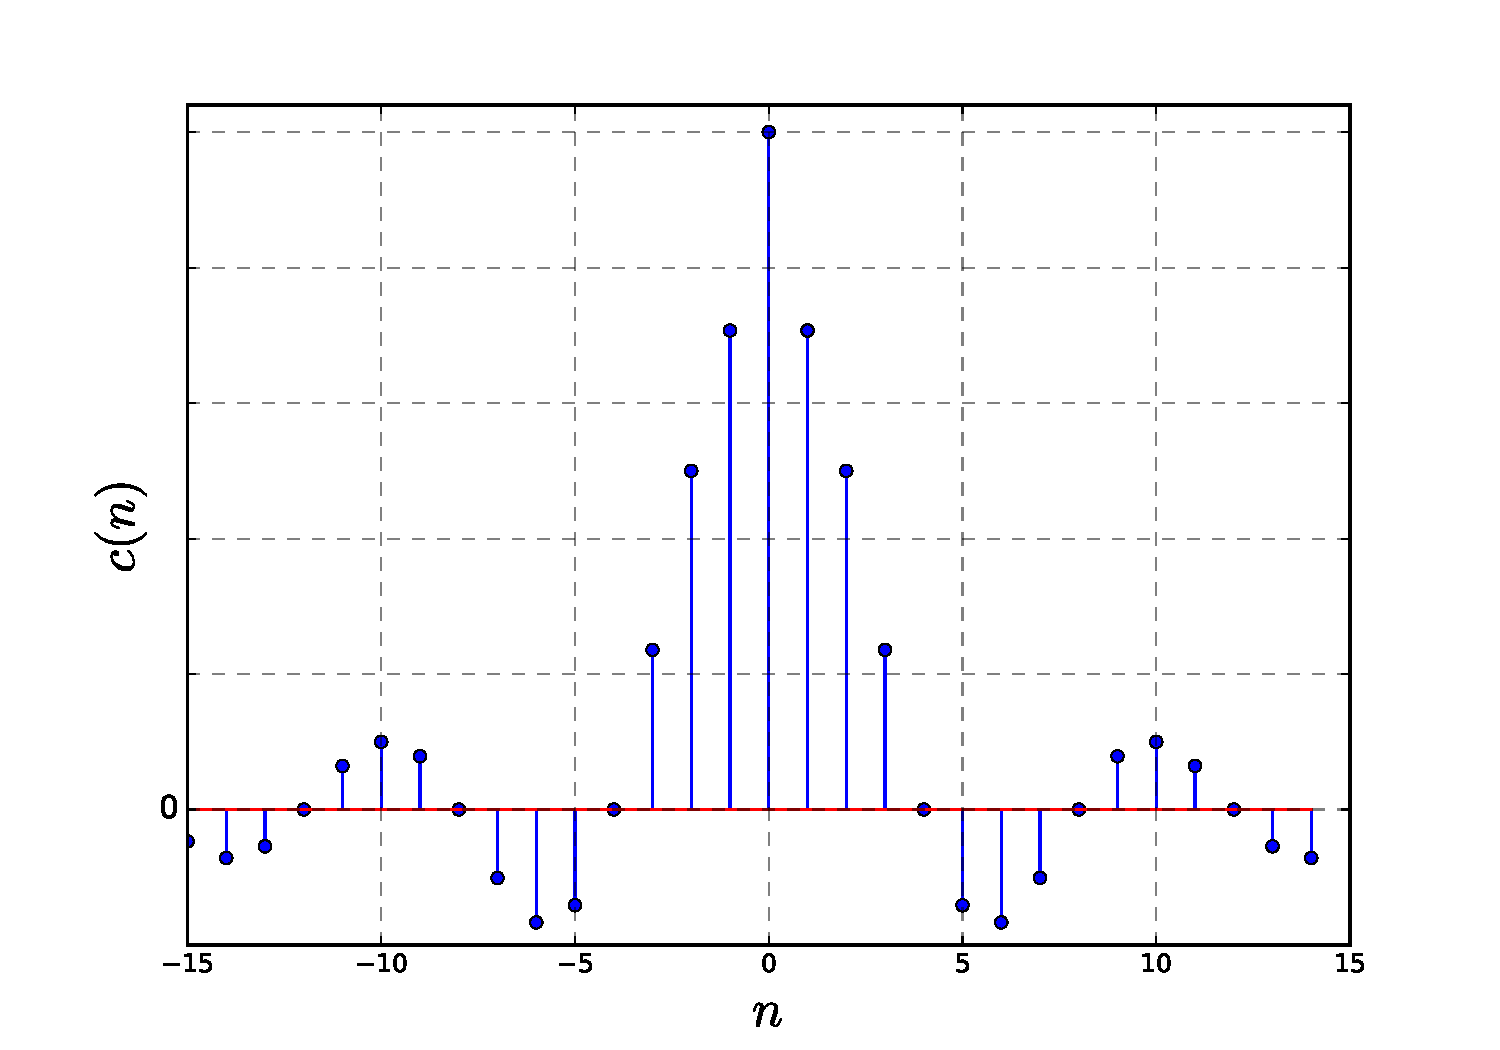
\includegraphics[scale = 0.4]{Figuras/Espectro1.pdf}
    \caption{Espectro de Fourier.}
\end{figure}

En lugar de graficar $c$ vs $n$, podemos graficar $c$ vs ``el número de onda" (frecuencia asociada a la parte espacial):
$$k = \frac{2\pi n}{L}.$$

Si $L \to \infty$, entonces las frecuencias se encuentran estrechamente espaciadas debido a que la diferencia entre valores consecutivos de $k$ es
$$\Delta k = \frac{ 2\pi \Delta n}{L}  = \frac{2\pi}{L}, \quad \mbox{pues}~ \Delta n = 1.$$

En otras palabras, para $L \to \infty$, $\Delta k$ es pequeño. Con este cambio de escala, el espectro de Fourier puede parecerse a lo mostrado en la figura \ref{Espectro1}.

\begin{figure}
    \centering
    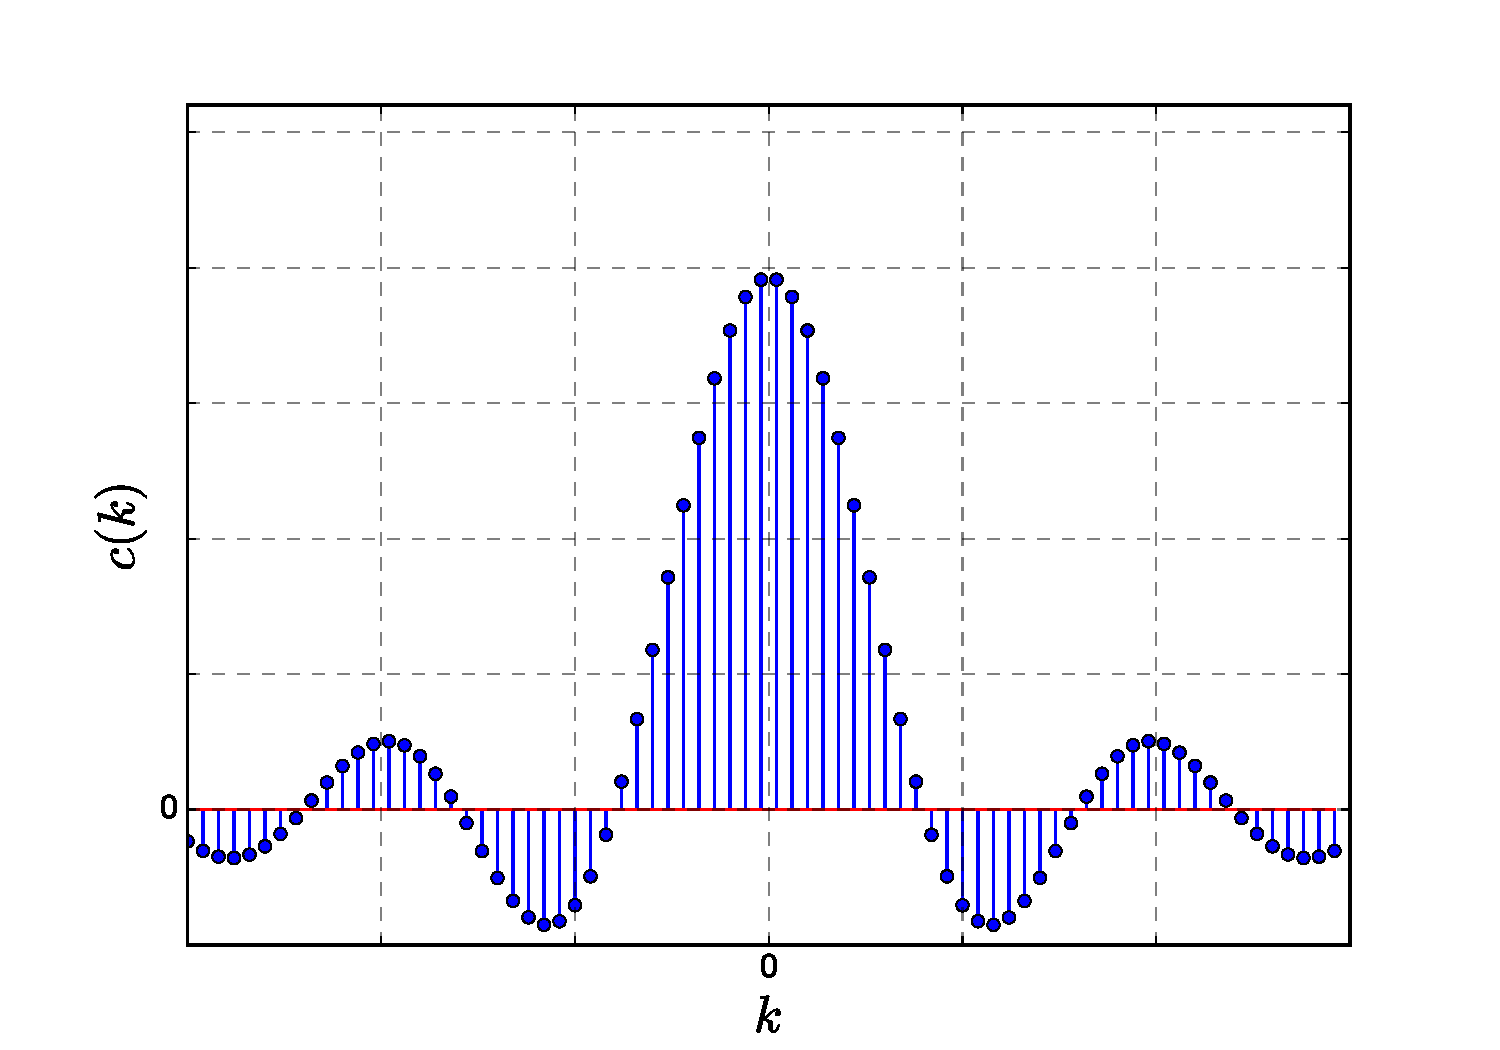
\includegraphics[scale = 0.4]{Figuras/Espectro2.pdf}    \caption{Espectro de Fourier cuando $L \to + \infty$.}
    \label{Espectro1}
\end{figure}

Es natural especular sobre la posibilidad de un espectro continuo cuando $L$ tiende al infinito  de tal forma que todas las frecuencias están presentes. Puede ser instructivo considerar la siguiente derivación heurística: Sabemos que una función puede ser expandida como una serie de Fourier tal como se muestra en \eqref{Transformada1}. Luego, la transición $L \to \infty$ puede resultar difícil de realizar directamente ya que $c_n$ aparentemente tiende a cero. Seguimos entonces la idea de usar las frecuencias $k = 2\pi n/L$ tal que
$\Delta k = (2\pi/L ) \Delta n = 2\pi/L$ para valores de $k$ adyacentes y definimos
$$c_L(k) = \frac{L}{2 \pi} c_n.$$

Usando las definiciones anteriores en las ecuaciones \eqref{Transformada1} y \eqref{Transformada2}, obtenemos: 
\begin{align*}
    f(x)&= \sum_{Lk/2\pi = -\infty}^{\infty} \frac{2\pi}{L} c_L(k) e^{ikx} \left( \frac{\Delta k L}{2\pi}\right) = \sum_{Lk/2\pi = -\infty}^{\infty}  c_L(k) e^{ikx} \Delta k , \\
  c_L(k) &= \frac{L}{2\pi} \frac{1}{L} \int_{-L/2}^{L/2} f(x) e^{-ikx} dx = \frac{1}{2\pi} \int_{-L/2}^{L/2} f(x) e^{-ikx} dx.
\end{align*}

Al hacer $L \to \infty$, la función $f$ puede considerarse como una
función no-periódica arbitraria definida en todo el intervalo $(-\infty, \infty)$ y  esperamos que la primera suma ``pase"  \text{a} una integral:
\begin{align*}
    f(x)&= \int_{-\infty}^{\infty} c(k) e^{ikx} \,dk, \\
  c(k) &= \lim_{L\to + \infty} c_L(k) =  \frac{1}{2\pi}  \int_{-\infty}^{\infty} f(x) e^{-ikx} dx.
\end{align*}

De aquí, definimos la \textbf{transformada de Fourier} de la función $f(x)$ como 
\begin{shaded}
  \begin{equation}
 \tilde{f}(k) := \frac{1}{2\pi} \int_{-\infty}^{\infty} f(x) e^{-ikx} dx \label{T.Fourier},
\end{equation}  
\end{shaded}

de modo que la ``transformada inversa" \, \text{resulta} ser
\begin{shaded}
  \begin{equation}
 f(x) =  \int_{-\infty}^{\infty} \tilde{f}(k) e^{ikx} \,dk. \label{I.Fourier}
\end{equation}  
\end{shaded}

 Note que la transformada de Fourier es la extensión natural del concepto de series de Fourier para funciones no periódicas. Además, al ser $n$ una variable discreta, y $k$ continua, podemos decir que la transformada de Fourier es la generalización del concepto de series de Fourier cuando las funciones pertenecen a un espacio vectorial de dimensión continua.

\textbf{Observaciones:}
\begin{itemize}
    \item Otras notaciones usadas son: $\tilde{f}(k) = g(k) = \mathcal{F}\{f(x)\}(k)$.
    
    \item El factor $1/2\pi$ en la definición \eqref{T.Fourier} es hasta cierto punto convencional. Lo importante es que se cumpla la identidad
    \begin{equation}
        f(x) = \int_{-\infty}^{\infty} \left[\frac{1}{2\pi} \int_{-\infty}^{\infty} f(\xi) e^{-ik\xi} d\xi \right] e^{ikx} \,dk.
      \label{IntegralFourier}
    \end{equation}
   
    Por ejemplo, en lugar de estos factores, podría introducirse un $\alpha$ en \eqref{I.Fourier} y $1/(2\pi \alpha)$ en \eqref{T.Fourier}, con $\alpha$ una constante arbitraria. Algunas elecciones populares son: $\alpha = 1$ y $\alpha = 1/\sqrt{2\pi}$ \cite{Rubilar}.

    \item Al igual que el factor $1/2\pi$ en la definición \eqref{T.Fourier}, la función $e^{-ikx}$ es convencional y puede ser reemplazada por $e^{ikx}$, siempre y cuando se verifique \eqref{IntegralFourier} \cite{Butkov, Riley}.
    
    \item En el caso que $f(x)$ sea real, tenemos que \eqref{IntegralFourier} se puede escribir como 
    \begin{equation}
        f(x) = \frac{1}{\pi} \int_{0}^{\infty} \int_{-\infty}^{\infty} f(\xi) \cos k(x-\xi)  \, d\xi \,dk.  \label{IntegralFourierReal}
    \end{equation}

    \colorlet{shadecolor}{blue!10} 
    \begin{shaded}
    En efecto, la relación \eqref{IntegralFourier} también se puede expresar como 
    $$f(x) = \frac{1}{2\pi}  \int_{-\infty}^{\infty} \int_{-\infty}^{\infty} f(\xi) e^{-ik\xi} e^{ikx} d\xi  \,dk = \frac{1}{2\pi}  \int_{-\infty}^{\infty} \int_{-\infty}^{\infty} f(\xi) e^{ik(x-\xi)} d\xi  \,dk.$$
    
    Como $f(x)$ es real, se igualan las partes reales para así obtener
    $$f(x) = \frac{1}{2\pi} \int_{-\infty}^{\infty} \int_{-\infty}^{\infty} f(\xi) \cos k(x-\xi) d\xi  \,dk. $$
    
    Puesto que $\cos k(x-\xi)$ es par con respecto a $k$, tenemos que 
    $$f(x) = \frac{2}{2\pi} \int_{0}^{\infty} \int_{-\infty}^{\infty} f(\xi) \cos k(x-\xi)  \, d\xi \,dk =\frac{1}{\pi} \int_{0}^{\infty} \int_{-\infty}^{\infty} f(\xi) \cos k(x-\xi)  \, d\xi \,dk. $$  
    \end{shaded}
    \colorlet{shadecolor}{green!20}
    
    \item Es común en Física trabajar con funciones del tiempo, $f = f(t)$. En este caso, se acostumbra usar la frecuencia $\omega$ en lugar del número de onda $k$, de modo que la integral de Fourier adopta a forma
    $$
    f(t) = \int_{- \infty}^{\infty} \Tilde{f}(\omega) e^{i \omega t} d\omega,
    $$

    donde
    $$
    \Tilde{f}(\omega) = \frac{1}{2\pi} \int_{- \infty}^{\infty} f(t) e^{- i \omega t} dt.
    $$
    
    \item En 3 dimensiones, la integral de Fourier está dada por:
    \begin{align*}
         f(\vec{r}\,) &:= \int_{\mathbb{R}^3} \tilde{f}(\vec{k}) e^{i (\vec{k} \cdot \vec{r})} d^3k, \\
         \tilde{f}(\vec{k}\,) &:= \frac{1}{(2\pi)^3} \int_{\mathbb{R}^3} f(\vec{r}) e^{-i (\vec{k} \cdot \vec{r})} d^3x.
    \end{align*}
    
    En general, en $n$ dimensiones:
     \begin{align*}
         f(\vec{r}\,) &:= \int_{\mathbb{R}^n} \tilde{f}(\vec{k}) e^{i (\vec{k} \cdot \vec{r})} d^n k, \\
         \tilde{f}(\vec{k}\,) &:= \frac{1}{(2\pi)^n} \int_{\mathbb{R}^n} f(\vec{r}) e^{-i (\vec{k} \cdot \vec{r})} d^n x.
    \end{align*}
   
\end{itemize}


\begin{defi}
Si $f(x)$ es tal que 
$$\int_{-\infty}^{\infty} |f(x)| \,dx < \infty,$$

entonces se dice que $f \in  L^1$ o que es \textbf{absolutamente integrable}.
\end{defi}

\begin{teorema}
Si $f \in L^1$, entonces la transformada de Fourier $\tilde{f}(k) = \mathcal{F}\{f(x)\}(k)$ existe y $\lim\limits_{k \to \pm \infty} \tilde{f}(k) = 0$.
\end{teorema}

\begin{demo}

Demostraremos solo la primera parte del teorema.

Notemos que
$$e^{-ikx} = \cos(kx) - i \sin(kx) ~\Rightarrow~ |e^{-ikx}| = 1.$$

Luego,
$$ \int_{-\infty}^{\infty} |f(x) e^{-ikx}| dx =  \int_{- \infty}^{\infty} |f(x)| \,dx < \infty.$$

En consecuencia, $f(x) e^{-ikx}$ es absolutamente integral y
$$\frac{1}{2\pi} \int_{-\infty}^{\infty} f(x) e^{-ikx} dx$$

es finita, es decir, $\tilde{f}(k)$ existe. 
\end{demo}

\textbf{Observación:} La condición de que $f$ sea absolutamente integrable es suficiente pero no necesaria para la existencia de la transformada de Fourier.

\begin{teorema}
    Sea $f(x)$ una función seccionalmente continua en cada intervalo finito del eje $x$, y supongamos que es absolutamente integrable en $(-\infty, + \infty)$. Entonces la \textbf{integral de Fourier}
$$
\frac{1}{\pi} \int_0^{+\infty} \int_{-\infty}^{+\infty} f(\xi) \cos k(\xi-x) \,d\xi dk = \frac{f(x^+) + f(x^-)}{2},
$$

donde ambas derivadas laterales, $f'(x^+)$ y $f'(x^-)$, existen.
\end{teorema}

\begin{demo}
Consulte el cápitulo 6 <<Fourier Integrals and Applications>> en \cite{Brown}.
\end{demo}

\section{Ejemplos}

\begin{ejemplo}[Pulso cuadrado] \label{PulsoCuadrado}
Consideremos la función 
$$f(x) = \left\{ \begin{array}{cl}
     1,& |x|<a  \\
     0,& |x|> a
\end{array} \right..$$

Su transformada de Fourier es 
\begin{align}
    \tilde{f}(k) = \frac{1}{2\pi} \int_{-\infty}^{\infty} f(x) e^{-ikx} dx &= \frac{1}{2\pi}\int_{-a}^a (1)  e^{-ikx} dx \nonumber \\
    &= \frac{1}{2\pi} \left[ - \frac{1}{ik} e^{-ikx} \right]_{-a}^a \nonumber\\
    &= \frac{1}{2\pi i k} [e^{ika} - e^{-ika}] \nonumber\\
    &= \frac{\sin(ka)}{\pi k}. \label{TransPulsoCuadrado}
\end{align}

\begin{figure}[H]
    \centering
    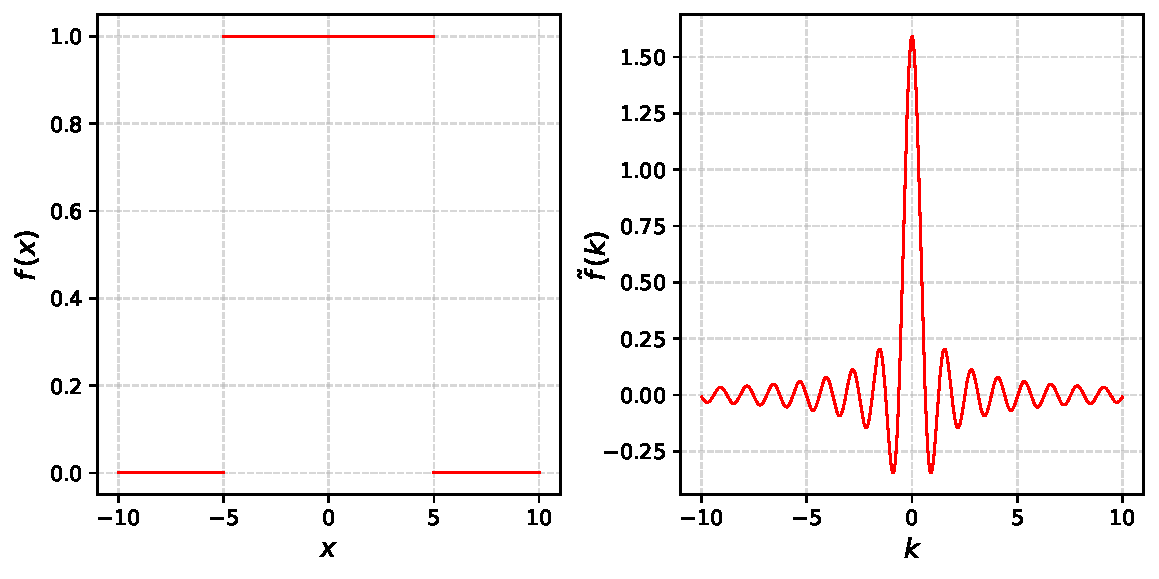
\includegraphics[scale = 0.55]{Figuras/EjemploTransformada1.pdf}
    \caption{Pulso cuadrado y su transformada de Fourier, con $a = 5$.}
    \label{Espectro2}
\end{figure}

\end{ejemplo}

\begin{ejemplo}[Distribución gaussiana]

Considere la gaussiana
$$f(x) = n e^{-\alpha x^2}, \quad  \alpha > 0.$$

Su transformada de Fourier está dada por 
\begin{equation*}
    \tilde{f}(k) =  \frac{n}{2\pi} \int_{-\infty}^{\infty} e^{-\alpha x^2} e^{-ikx} dx =  \frac{n}{2\pi} \int_{-\infty}^{\infty} e^{-\alpha x^2-ikx} dx .
\end{equation*}

Notemos que 
\begin{align*}
    -\alpha x^2-ikx &= - \alpha \left( x^2 + \frac{ik}{\alpha}x \right) \\
    &= - \alpha \left( x^2 + \frac{ik}{\alpha} x + \left( \frac{ik}{2\alpha} \right)^2 - \left( \frac{ik}{2\alpha} \right)^2 \right) \\
    &= - \alpha \left( x + \frac{ik}{2\alpha} \right)^2 + \alpha \left( \frac{ik}{2\alpha} \right)^2 \\
    &= - \alpha \left( x + \frac{ik}{2\alpha} \right)^2 - \left( \frac{k^2}{4\alpha} \right).
\end{align*}

Luego, 
\begin{equation*}
    \tilde{f}(k) =  \frac{n}{2\pi} \int_{-\infty}^{\infty} e^{-\alpha \left( x + \frac{ik}{2\alpha} \right)^2 - \left( \frac{k^2}{4\alpha} \right)}  dx = \frac{n}{2\pi} e^{- \left( \frac{k^2}{4\alpha} \right)} \int_{-\infty}^{\infty} e^{-\alpha \left( x + \frac{ik}{2\alpha} \right)^2} \,dx. 
\end{equation*}

Probaremos, usando las herramientas que nos brinda el Cálculo Complejo, que
$$
 \int_{-\infty}^{\infty} e^{-\alpha \left( x + \frac{ik}{2\alpha} \right)^2} \,dx =  \int_{-\infty}^{\infty} e^{- \alpha x^2} dx.
$$

Consideremos la integral 
\begin{equation}
   \int_{\gamma} e^{-\alpha \left( z + \frac{ik}{2\alpha} \right)^2} dz \label{IntegralComplexGauss} 
\end{equation}

donde el contorno $\gamma$ es un rectángulo que está ilustrado en la figura \ref{fig:ContornoGauss}.

\begin{figure}[H]
    \centering
    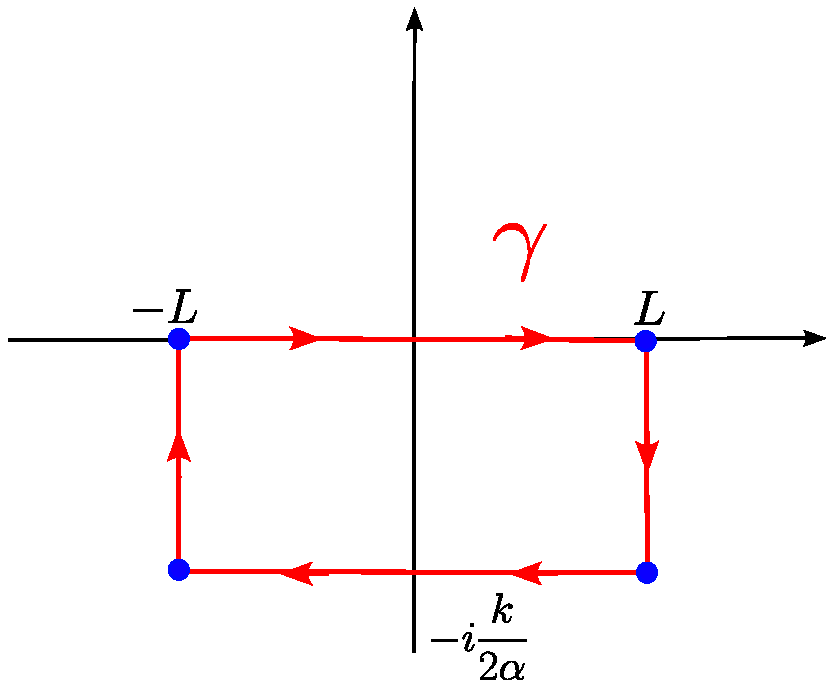
\includegraphics[scale = 0.53]{Figuras/ContornoFourierGauss.pdf}
    \caption{Contorno cerrado orientado positivamente, $\gamma$, constituido por la unión del segmento dirigido de $-L$ a $L$, de $L$ a $L - ik/2\alpha$, de $L - ik/2\alpha$ a $-L - ik/2\alpha$ y de $-L - ik/2\alpha$ a $-L$.}
    \label{fig:ContornoGauss}
\end{figure}

Como el integrando no tiene singularidades dentro del rectángulo, entonces por el teorema de Cauchy-Goursat, la integral \eqref{IntegralComplexGauss} es igual a cero. Así, evaluando la integral en cada segmento,
\begin{align*}
 \int_{\gamma} e^{-\alpha \left( z + \frac{ik}{2\alpha} \right)^2} dz &= \int_{-L}^L e^{-\alpha \left( x + \frac{ik}{2\alpha} \right)^2} dx + \int_0^{- \frac{k}{2\alpha}} i e^{-\alpha \left( L + i \left( y + \frac{k}{2\alpha} \right) \right)^2} dy   \\
 & \quad - \int_{-L}^L e^{-\alpha x^2} dx + \int_{- \frac{k}{2\alpha}}^0 i e^{-\alpha \left(- L + i \left( y + \frac{k}{2\alpha} \right) \right)^2} dy = 0.
\end{align*}

La segunda y cuarta integral, al lado derecho de la igualdad, se anulan cuando $L \to + \infty$. Luego,
$$\lim_{L \to + \infty} \int_{-L}^L e^{-\alpha \left( x + \frac{ik}{2\alpha} \right)^2} dx = \lim_{L \to + \infty} \int_{-L}^L e^{-\alpha x^2} dx.$$

Pero, las integrales
$$\int_{- \infty}^{\infty} e^{-\alpha \left( x + \frac{ik}{2\alpha} \right)^2} dx ~~\mbox{y}~~ \int_{-\infty}^{\infty} e^{-\alpha x^2} dx$$

convergen (¿Por qué?), entonces sus valores coinciden con su valor principal de Cauchy. Por lo tanto,
$$\int_{-\infty}^{\infty} e^{-\alpha \left( x + \frac{ik}{2\alpha} \right)^2} \,dx = \lim_{L \to + \infty} \int_{-L}^L e^{-\alpha \left( x + \frac{ik}{2\alpha} \right)^2} dx = \lim_{L \to + \infty} \int_{-L}^L e^{-\alpha x^2} dx = \int_{-\infty}^{\infty} e^{-\alpha x^2} \,dx.$$

Volviendo al cálculo de la transformada de Fourier,
$$
\Tilde{f}(k) = \frac{n}{2\pi} e^{- \left( \frac{k^2}{4\alpha} \right)} \int_{-\infty}^{\infty} e^{-\alpha x^2} \,dx.
$$

Como
$$\int_{-\infty}^{\infty} e^{-\alpha x^2} \,dx = \sqrt{\frac{\pi}{\alpha}}, \quad \alpha > 0$$

obtenemos que 
$$\tilde{f}(k) = \frac{n}{2\pi}\sqrt{\frac{\pi}{\alpha}}e^{- \left( \frac{k^2}{4\alpha} \right)}.$$

\begin{figure}[H]
    \centering
    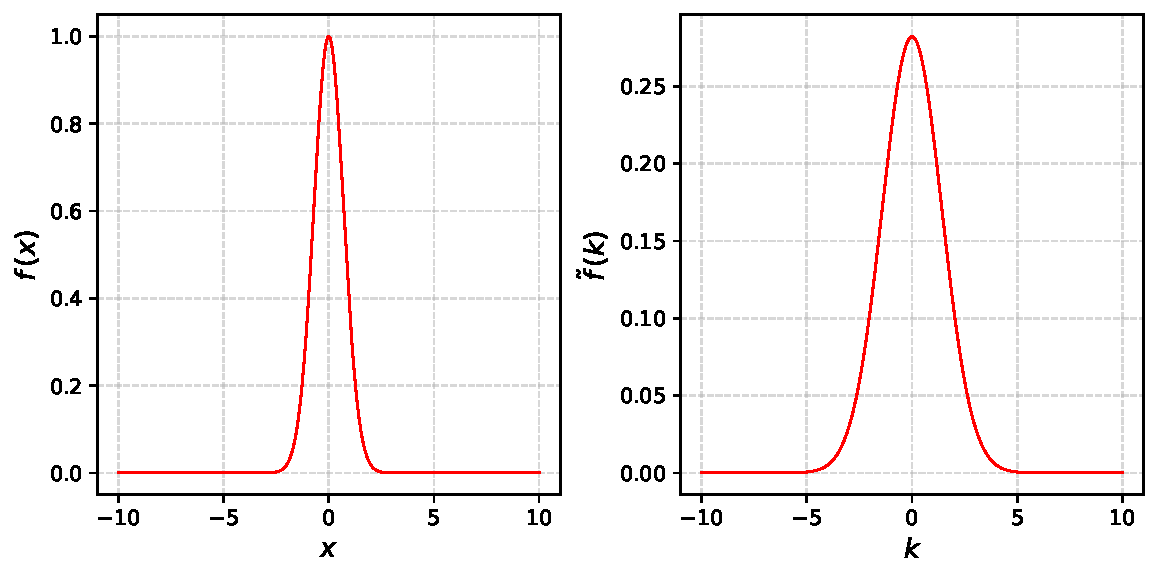
\includegraphics[scale = 0.6]{Figuras/EjemploTransformada2.pdf}
    \caption{Distribución gaussiana y su transformada de Fourier para $n=1$ y $\alpha =1$ .}
    \label{Espectro3}
\end{figure}

\begin{figure}[H]
    \centering
    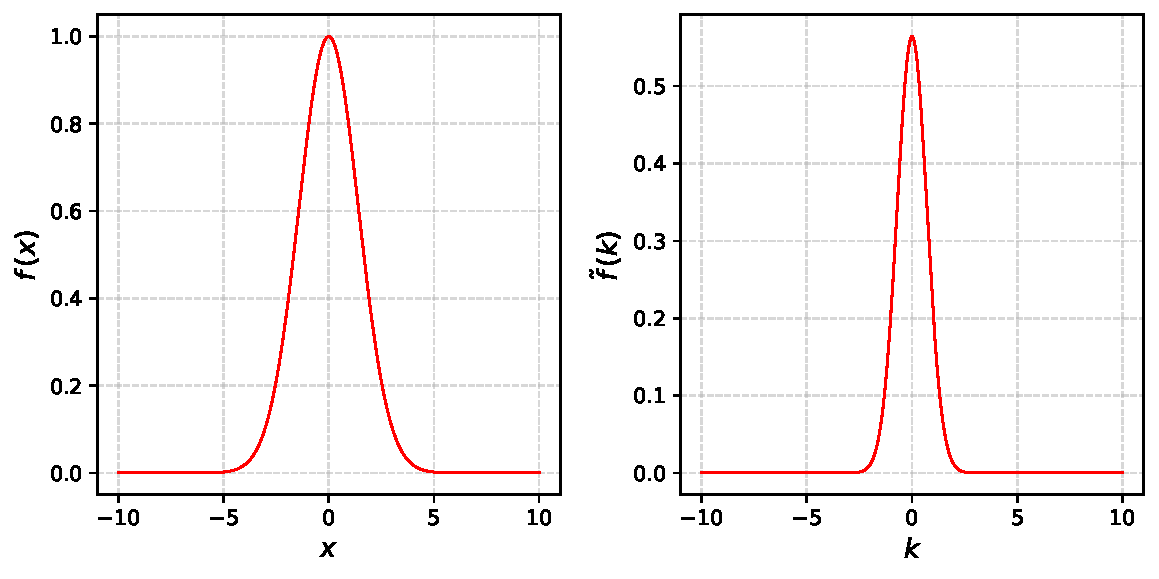
\includegraphics[scale = 0.6]{Figuras/EjemploTransformada3.pdf}
    \caption{Distribución gaussiana y su transformada de Fourier para $n=1$ y $\alpha =0.25$ .}
    \label{Espectro4}
\end{figure}
\end{ejemplo}

\begin{ejemplo}[Paridad]
Si $f(x) \in \mathbb{R}$ e impar, entonces
\begin{align*}
     \tilde{f}(k) &= \frac{1}{2\pi} \int_{-\infty}^{\infty} f(x) e^{-ikx} dx \\
&= \frac{1}{2\pi} \int_{-\infty}^0 f(x) e^{-ikx} \,dx + \frac{1}{2\pi} \int_{0}^{\infty} f(x) e^{-ikx} \, dx  \\
 &= -\frac{1}{2\pi} \int_{\infty}^0 f(-x) e^{ikx} \,dx + \frac{1}{2\pi} \int_{0}^{\infty} f(x) e^{-ikx} \, dx \\
     &= -\frac{1}{2\pi} \int_{0}^{\infty} f(x) e^{ikx} \,dx + \frac{1}{2\pi} \int_{0}^{\infty} f(x) e^{-ikx} \, dx  \\
      &= -\frac{1}{2\pi} \int_{0}^{\infty} f(x) [e^{ikx} - e^{-ikx}  ] \,dx \\
     &= -\frac{2i}{2\pi} \int_{0}^{\infty} f(x) \sin(kx) \,dx \equiv - i  \tilde{f}_S(k),
     \end{align*}
     
     donde $\tilde{f}_S$ es conocida como la \textbf{transformada seno de Fourier} de la función $f(x)$, y viene definida por \cite{Mauch} 
     $$\boxed{\tilde{f}_S(k) = \frac{1}{\pi}  \int_{0}^{\infty} f(x) \sin(kx) \,dx}$$
     
Análogamente a la definición de la  transformada seno de Fourier, si $f(x) \in \mathbb{R}$ y par, entonces 
\begin{align*}
     \tilde{f}(k) = \frac{1}{2\pi} \int_{-\infty}^{\infty} f(x) e^{-ikx} dx &= \frac{1}{2\pi} \int_{-\infty}^0 f(x) e^{-ikx} \,dx + \frac{1}{2\pi} \int_{0}^{\infty} f(x) e^{-ikx} \, dx  \\
     &= -\frac{1}{2\pi} \int_{\infty}^0 f(-x) e^{ikx} \,dx + \frac{1}{2\pi} \int_{0}^{\infty} f(x) e^{-ikx} \, dx \\
     &= \frac{1}{2\pi} \int_{0}^{\infty} f(x) e^{ikx} \,dx + \frac{1}{2\pi} \int_{0}^{\infty} f(x) e^{-ikx} \, dx \\
     &= \frac{1}{2\pi} \int_{0}^{\infty} f(x) [e^{ikx} + e^{-ikx}  ] \,dx \\
     &= \frac{2}{2\pi} \int_{0}^{\infty} f(x) \cos(kx) \,dx \equiv  \tilde{f}_C(k),
     \end{align*}
     
donde $\tilde{f}_C$ es conocida como la \textbf{transformada coseno de Fourier} de la función $f(x)$, y viene definida por \cite{Mauch}
     $$\boxed{\tilde{f}_C(k) = \frac{1}{\pi}  \int_{0}^{\infty} f(x) \cos(kx) \,dx}$$

\textbf{Observación: } Esta forma de escribir la transformada seno y coseno de Fourier es convencional, por el factor $1/\pi$.
\end{ejemplo}

\begin{comment}
\begin{ejemplo}
Consideremos ahora una función $f(x) \notin L^1$. Sea $f(x) = \sign(x)$  tal que $f(x) \notin L^1$, ya que $\int\limits_{-\infty}^{\infty}  |f(x)| \,dx$ diverge. Intentemos de todas maneras evaluar la transformada de Fourier, teniendo en cuenta que $f$ es real e impar.

\begin{align*}
    \tilde{f}(k) = \frac{1}{2\pi} \int_{-\infty}^{\infty} \sign(x) e^{-ikx} \,dx &= -\frac{i}{\pi} ^*\int_{0}^{\infty} \sin kx \,dx \qquad \mbox{(Integral de Cesàro)} \\
    &= \left\{ \begin{array}{cl}
        \frac{1}{i \pi k},  & k \neq 0  \\
         0, & k = 0
    \end{array} \right. .
\end{align*}

\end{ejemplo}    
\end{comment}

\section{Propiedades de la transformada de Fourier}

\begin{propo}
Sean $f, g \in L^1$ y $\alpha, \beta \in \mathbb{C}.$

\begin{enumerate}
    \item \textbf{Linealidad}: $$\mathcal{F}\{\alpha f(x) + \beta g(x)\}(k) = \alpha \mathcal{F}\{f(x)\}(k) + \beta \mathcal{F}\{g(x)\}(k).$$ 
    
    \item Si $f$ es real, entonces $$ \mathcal{F}\{f(x)\}(-k) = (\mathcal{F}\{f(x)\}(k))^*.$$
    
    \item \textbf{Desplazamiento}: $$\mathcal{F}\{f(x+a)\}(k) = e^{ika} \mathcal{F}\{f(x)\}(k), \quad a \in \mathbb{R}.$$
    
    \item  \textbf{Atenuación}: $$\mathcal{F}\{f(x)e^{-ax}\}(k) =  \mathcal{F}\{f(x)\}(k-ia), \quad a \in \mathbb{C}.$$
\end{enumerate}
\end{propo}

\begin{demo}
A modo de ejemplo, se demostrará los puntos 1. y 2., el resto se encontrará en el documento extra de las demostraciones del apunte. 

\begin{enumerate}
    \item Por la definición \eqref{T.Fourier} de la transformada de Fourier y usando el hecho de que las funciones son absolutamente convergentes, tenemos
    \begin{align*}
        \mathcal{F}\{\alpha f(x) + \beta g(x)\}(k) &= \frac{1}{2\pi} \int_{-\infty}^{\infty} [\alpha f(x) + \beta g(x)] e^{-ikx} dx \\
        &= \frac{\alpha}{2\pi} \int_{-\infty}^{\infty}  f(x) e^{-ikx} dx + \frac{\beta}{2\pi} \int_{-\infty}^{\infty}  g(x) e^{-ikx} dx \\
        &= \alpha \mathcal{F}\{f(x)\}(k) + \beta \mathcal{F}\{g(x)\}(k).
    \end{align*}
    
    \item Por la definición \eqref{T.Fourier} de la transformada de Fourier y suponiendo que $f$ es real:
    \begin{align*}
        \mathcal{F}\{f(x)\}(-k) &= \frac{1}{2\pi} \int_{-\infty}^{\infty}  f(x)  e^{-(-ikx)} dx  \\
        &= \frac{1}{2\pi} \int_{-\infty}^{\infty}  f(x)  (e^{-ikx})^* dx  \\
        &= \frac{1}{2\pi} \int_{-\infty}^{\infty}  [f(x)  e^{-ikx}]^* dx \\
        &= (\mathcal{F}\{f(x)\}(k))^*.
    \end{align*}
\end{enumerate}
\end{demo}

\begin{propo}
Sea $f(x)$ con transformada de Fourier $\mathcal{F}\{f(x)\}$ y $\lim\limits_{x \to \pm \infty} f(x) = 0$. Entonces, 
$$\boxed{\mathcal{F}\{f'(x)\} = i k \mathcal{F}\{f(x)\}}$$
\end{propo}

\begin{demo}
Usando la definición \eqref{T.Fourier} de la transformada de Fourier, tenemos que 
\begin{align*}
    \mathcal{F}\{f'(x)\} &= \frac{1}{2\pi} \int_{- \infty}^{\infty} f'(x) e^{-ikx} \,dx \\
    &= \frac{1}{2\pi} \int_{- \infty}^{\infty} \left\{ \frac{d}{dx}\left[ f(x) e^{-ikx} \right]  - (-ik) f(x) e^{-ikx} \right\}\,dx \\
    &= \frac{1}{2\pi} \left. f(x) e^{-ikx} \right|_{-\infty}^{\infty} + \frac{ik}{2\pi} \int_{- \infty}^{\infty}  f(x) e^{-ikx} \,dx \\
    &=  ik \mathcal{F}\{f(x)\} + \left. f(x) e^{-ikx} \right|_{-\infty}^{\infty}.
\end{align*}

Como  $\lim\limits_{x \to \pm \infty} f(x) = 0$, obtenemos
$$\mathcal{F}\{f'(x)\} = i k \mathcal{F}\{f(x)\}.$$
\end{demo}

En general,
\begin{shaded}
$$\mathcal{F}\{f^{(n)} (x)\} = (i k)^n \mathcal{F}\{f(x)\},$$    
\end{shaded}

siempre que todas las partes integradas se anulen cuando $x \to \pm \infty$.

\begin{teorema}[de Parseval]
Si $f(x)$ y $g(x)$ son funciones reales y si $\tilde{f}(k)$ y $\tilde{g}(k)$ son sus correspondientes transformadas de Fourier, entonces

\begin{itemize}
    \item[(i)] (Primer teorema)
    $$\int_{-\infty}^{\infty} |\tilde{f}(k)|^2\, dk = \frac{1}{2\pi} \int_{-\infty}^{\infty} |f(x)|^2 \, dx. $$
    
    \item[(ii)] (Segundo teorema)
    $$\int_{-\infty}^{\infty} \tilde{f}(k) \tilde{g}(-k) \, dk = \frac{1}{2\pi} \int_{-\infty}^{\infty} f(x) g(x) \, dx. $$
    
\end{itemize}
\end{teorema}

\begin{demo}
Notemos que (i) es consecuencia de (ii) al tomar $g(x) = f(x)$ real tal que $f^*(x) = f(x)$ y $\tilde{g}(-k) = \tilde{f}^*(k)$. Luego, nos bastará demostrar el segundo teorema de Parseval.

Usando la definición \eqref{T.Fourier}, tenemos que 
$$\tilde{g}(-k) = \frac{1}{2\pi} \int_{-\infty}^{\infty} g(x) e^{ikx} \,dx.$$

Luego, 
$$\int_{-\infty}^{\infty} \tilde{f}(k) \tilde{g}(-k) \,dk = \int_{-\infty}^{\infty} \tilde{f}(k) \,dk \int_{-\infty}^{\infty} \frac{1}{2\pi} g(x) e^{ikx} \,dx.$$

Supongamos que podemos intercambiar el orden de integración, por ejemplo, al suponer que las integrales 
$$\int_{-\infty}^{\infty} \tilde{f}(k) e^{ikx} \,dk ~~\mbox{y}~~ \int_{-\infty}^{\infty} g(x) e^{ikx} \,dx$$

son absolutamente integrables. Entonces,
$$\int_{-\infty}^{\infty} \tilde{f}(k) \tilde{g}(-k) \,dk = \frac{1}{2\pi} \int_{-\infty}^{\infty} g(x) \left(  \int_{-\infty}^{\infty}  \tilde{f}(k) e^{ikx} \,dk\right) \,dx.$$

Ahora, aplicando la transformada inversa de Fourier dada por \eqref{I.Fourier}, concluimos que
$$\int_{-\infty}^{\infty} \tilde{f}(k) \tilde{g}(-k) \,dk = \frac{1}{2\pi} \int_{-\infty}^{\infty} f(x) g(x)  \,dx.$$

\end{demo}

\begin{ejemplo}
    Use el teorema de Parseval para evaluar
    $$\int_{-\infty}^{\infty}  \frac{\sin^2(x)}{x^2} \,dx.$$

    \textbf{Solución:} Esta integral puede ser calculada usando el teorema del residuo. En nuestro caso, usaremos el primer teorema de Parseval, teniendo en cuenta el resultado de la transformada de Fourier del pulso cuadrado en el ejemplo \ref{PulsoCuadrado}. 

    Para $a = 1$ en la ecuación \eqref{TransPulsoCuadrado}, tenemos que
    $$\int_{- \infty}^{\infty} |\Tilde{f}(k)|^2 \,dk = \int_{- \infty}^{\infty} \frac{\sin^2(k)}{\pi^2 k^2}  \,dk = \frac{1}{\pi^2} \int_{-\infty}^{\infty}  \frac{\sin^2(k)}{k^2} \,dk.$$

    Por el primer teorema de Parseval,
    \begin{align*}
        \int_{- \infty}^{\infty} |\Tilde{f}(k)|^2 \,dk &= \frac{1}{2\pi} \int_{-\infty}^{\infty} |f(x)|^2 \,dx \\
        \Rightarrow \frac{1}{\pi^2} \int_{-\infty}^{\infty}  \frac{\sin^2(k)}{k^2} &= \frac{1}{2\pi} \int_{-1}^1 \,dx = \frac{1}{\pi}. 
    \end{align*}

Por lo tanto,
$$\int_{-\infty}^{\infty}  \frac{\sin^2(k)}{k^2} \,dk = \pi.$$
\end{ejemplo}

\section{Convolución}

\begin{defi}
Sean $f(x)$ y $g(x)$ dos funciones reales, se define la operación \textbf{convolución} de dos funciones $f$ y $g$ como 
\begin{equation}
 (f*g)(x) := \int_{-\infty}^{\infty} f(y) g(x-y) \,dy.   \label{Convolucion}
\end{equation}

\end{defi}

\textbf{Idea física:} Sea $f(t)$ algún ``estímulo" (fuerza en el tiempo $t$, densidad de carga en la posición $x$, etc). Sea $g(x,t) = g(x-t)$ la respuesta en $x$ a un estímulo en $t$. Si el sistema es \textit{lineal}, la respuesta total en el punto $x$ al estímulo global $\{f(t) : t \in \mathbb{R}\}$ será la "suma" de todas las contribuciones $[dt\, f(t)] g(x,t)$, que es la convolución $(f*g)(x)$. 

Por ejemplo, el potencial electrostático debido a una densidad de carga $\rho(\Vec{x})$ se puede escribir como
$$\phi(\Vec{x}) = \int_{V} \frac{\rho(\Vec{x}\,')}{|\Vec{x} - \Vec{x}\,'|} \, dV' = \rho * f(\Vec{x}),$$

donde  $f(\Vec{x}) = 1/|\Vec{x}|$.

\begin{figure}[H]
    \centering
    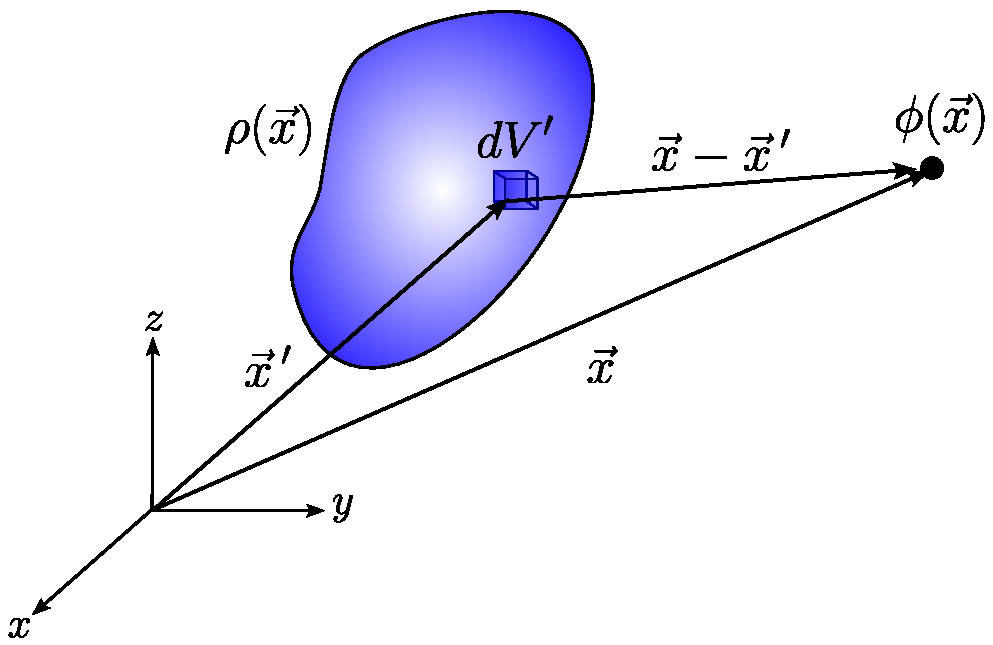
\includegraphics[scale = 0.55]{Figuras/Distribucion-Cargas.pdf}
    \caption{Distribución de carga de densidad $\rho(\Vec{x})$.}
    \label{fig:PotencialDistribucion}
\end{figure}

\textbf{Idea matemática:} La interpretación matemática de la convolución está ilustrada en la figura \ref{fig:IdeaConvolucion}.

\begin{figure}[H]
    \centering
    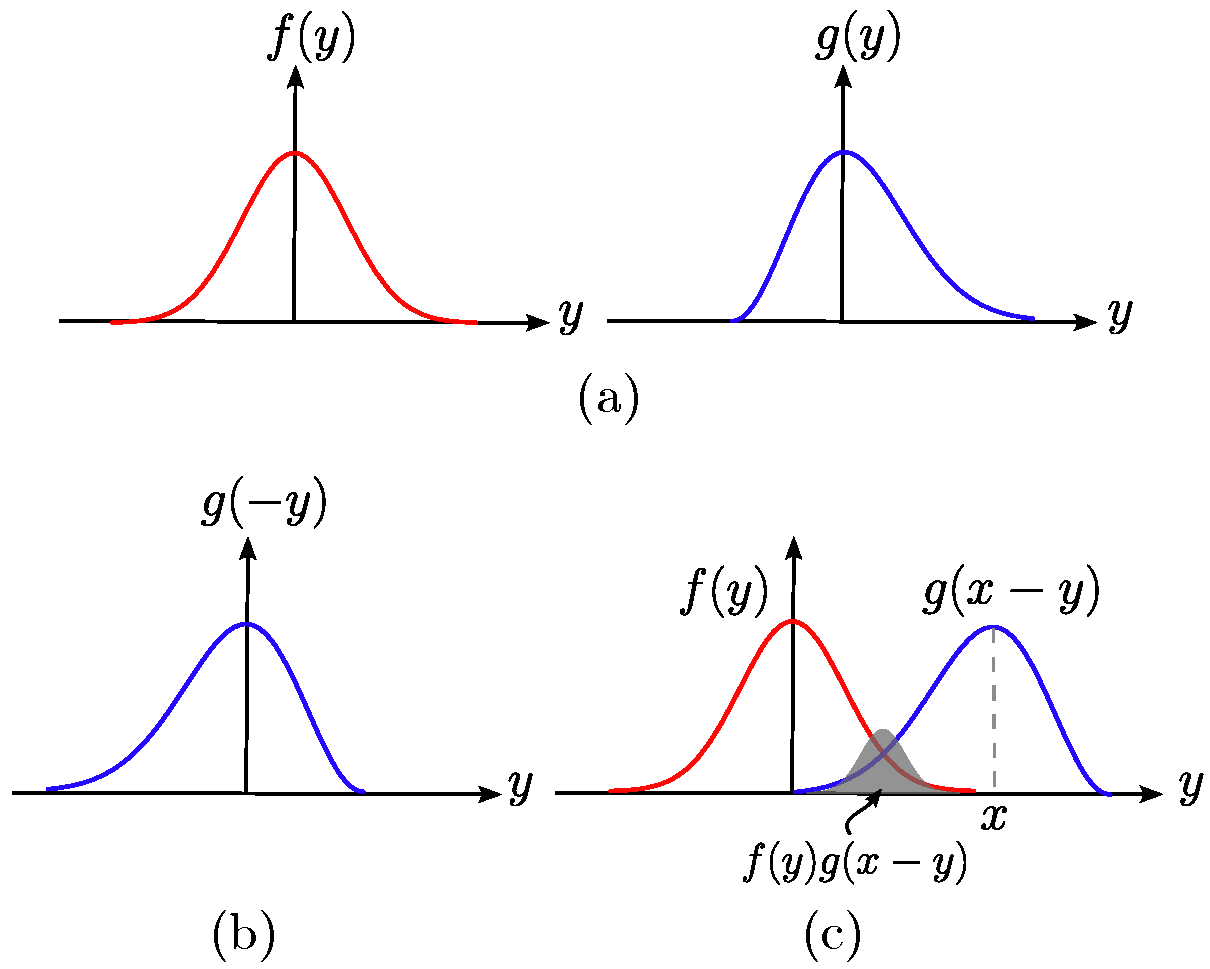
\includegraphics[scale = 0.55]{Figuras/Idea-Convolucion.pdf}
    \caption{Idea matemática de la convolución. En (a), se expresa cada función en términos de la variable de integración $y$. En (b), se refleja la gráfica de $g(y)$ con respecto al eje vertical, es decir, $g(y) \rightarrow g(-y)$. En (c), se traslada la gráfica de $g(-y)$, $x$ unidades. Luego, se traslapan las gráficas de $f(y)$ y $g(x-y)$ de tal forma que el área sombreada corresponde al valor de $f * g$ para ese valor de $x$.}
    \label{fig:IdeaConvolucion}
\end{figure}

Entonces, $f * g$ mide el grado de traslape entre $f(y)$ y $g(-y)$, luego de trasladar $g$ a una distancia $x$.

\begin{propo}[Propiedades de la convolución]
Sean $f(x)$, $g(x)$ y $h(x)$  funciones reales, se verifica:

\begin{enumerate}
    \item \textbf{Conmutatividad:}$$f(x) * g(x) = g(x) * f(x).$$
    
    \item \textbf{Asociatividad:} $$[f(x)*g(x)]*h(x) = f(x)*[g(x)*h(x)].$$
    
    \item \textbf{Distributividad:} $$f(x)*[g(x)+h(x)] = f(x)*g(x) + f(x)*h(x).$$ 
\end{enumerate}
\end{propo}

\newpage

\begin{teorema}[de convolución de Fourier]
Sean $f(x)$, $g(x)$ y $h(x)$  funciones reales y sean $\tilde{f}(k)$, $\tilde{g}(k)$ y $\tilde{h}(k)$ sus correspondientes transformadas de Fourier. 

\begin{itemize}
    \item Si $\tilde{h}(k) = \tilde{f}(k) \tilde{g}(k)$, entonces 
$$ h(x) = \frac{1}{2\pi} (f * g)(x) = \frac{1}{2\pi} (g * f)(x) = \frac{1}{2\pi} \int_{-\infty}^{\infty} f(y) g(x-y) \,dy.$$ 

    \item Si $h(x) = f(x) g(x)$, entonces
$$\Tilde{h}(k) = (\Tilde{f} * \Tilde{g})(k) = (\Tilde{g} * \Tilde{f})(k) = \int_{-\infty}^{\infty} \Tilde{f}(y) \Tilde{g}(k-y) \,dy.$$
\end{itemize}
\end{teorema}

\begin{demo}
\ 

\begin{itemize}
    \item Supongamos que  $\tilde{h}(k) = \tilde{f}(k) \tilde{g}(k)$. Aplicando la transformada de Fourier inversa dada por \eqref{I.Fourier}, tenemos que 
\begin{align*}
   h(x) = \mathcal{F}^{-1} \{\tilde{h}(k)\} &=  \mathcal{F}^{-1} \{\tilde{f}(k) \tilde{g}(k)\} \\
   &= \int_{-\infty}^{\infty} \tilde{f}(k) \tilde{g}(k) e^{ikx} \,dk \\
   &= \frac{1}{2\pi} \int_{-\infty}^{\infty}  \left( \int_{-\infty}^{\infty} f(y) e^{-ik y} \,dy \right) \tilde{g}(k)  e^{ikx}  \,dk.
\end{align*}

Si el intercambio de orden de integración es posible, entonces 
\begin{align*}
  h(x) &= \frac{1}{2\pi} \int_{-\infty}^{\infty}  f(y)  \left( \int_{-\infty}^{\infty}  \tilde{g}(k)  e^{ikx} e^{-ik y}\,d k \right) \,dy \\
   &= \frac{1}{2\pi} \int_{-\infty}^{\infty}  f(y)  \left( \int_{-\infty}^{\infty}  \tilde{g}(k)  e^{ik(x-y)}\,d k \right) \,dy \\
   &= \frac{1}{2\pi} \int_{-\infty}^{\infty}  f(y) g(x-y) \,dy = \frac{1}{2\pi} (f * g)(x).
\end{align*}

Como la convolución es conmutativa:
$$h(x) = \frac{1}{2\pi} (f * g)(x) = \frac{1}{2\pi} (g * f)(x)  = \frac{1}{2\pi} \int_{-\infty}^{\infty}  f(y) g(x-y) \,dy.$$

\item  Supongamos que $h(x) = f(x) g(x)$. Aplicando la transformada de Fourier dada por \eqref{T.Fourier}, tenemos que 
\begin{align*}
   \Tilde{h}(k) &=  \mathcal{F} \{f(x) g(x)\} \\
   &= \frac{1}{2\pi} \int_{-\infty}^{\infty} f(x) g(x) e^{-ikx} \,dx \\
   &=  \frac{1}{2\pi} \int_{-\infty}^{\infty} \left( \int_{-\infty}^{\infty} \Tilde{f}(y) e^{iyx} \,dy \right) g(x) e^{-ikx} \,dx.
\end{align*}

Si el intercambio de orden de integración es posible, entonces 
\begin{align*}
   \Tilde{h}(k) &=  \frac{1}{2\pi} \int_{-\infty}^{\infty} \Tilde{f}(y) \left( \int_{-\infty}^{\infty} g(x) e^{iyx}  e^{-ikx}\,dx \right) \,dy \\
   &=  \int_{-\infty}^{\infty} \Tilde{f}(y) \left( \frac{1}{2\pi} \int_{-\infty}^{\infty} g(x) e^{-i(k-y)x} \,dx \right) \,dy \\
   &=  \int_{-\infty}^{\infty} \Tilde{f}(y) \Tilde{g}(k-y) \,dy. 
\end{align*}

Por lo tanto,
$$\Tilde{h}(k) =  (\Tilde{f} * \Tilde{g})(k) = (\Tilde{g} * \Tilde{f})(k) = \int_{-\infty}^{\infty} \Tilde{f}(y) \Tilde{g}(k-y) \,dy.$$
\end{itemize}

\end{demo}


\begin{ejemplo}
    Sabiendo que \cite{Mauch}
    $$\mathcal{F}\left\{ \frac{2c}{x^2+c^2} \right\} = e^{-c|k|}, \quad \text{para} ~ c > 0.$$

    Podemos usar el teorema de convolución para encontrar la transformada de Fourier de
    \begin{equation}
      f(x) = \frac{1}{x^4+5x^2+4} = \frac{1}{(x^2+1)(x^2+4)}.    \label{EjConvo}
    \end{equation}
  
    En efecto,
    \begin{align*}
        \mathcal{F}\{f(x)\} &=  \mathcal{F}\left\{ \frac{1}{8} \frac{2}{x^2+1} \frac{4}{x^2+4} \right\} \\
        &= \frac{1}{8} \left( \int_{-\infty}^{\infty} e^{-|y|}e^{-2|k-y|} dy \right) \\
        &= \frac{1}{8} \left( \int_{-\infty}^0 e^{y}e^{-2|k-y|} dy +   \int_0^{\infty} e^{-y}e^{-2|k-y|} dy \right).
    \end{align*}

Si $k > 0$,
\begin{align*}
    \mathcal{F}\{f(x)\} &= \frac{1}{8} \left(  \int_{-\infty}^0 e^{y}e^{-2(k-y)} dy +  \int_0^k e^{-y}e^{-2(k-y)} dy + \int_k^{\infty} e^{-y}e^{2(k-y)} dy \right)  \\
    &= \frac{1}{8} \left(  \int_{-\infty}^0 e^{-2k+3y} dy +  \int_0^k e^{-2k+y} dy + \int_k^{+\infty} e^{2k-3y} dy \right) \\
    &= \frac{1}{8} \left( \frac{1}{3} e^{-2k} + e^{-k} - e^{-2k} + \frac{1}{3} e^{-k} \right) \\
    &= \frac{1}{6} e^{-k} - \frac{1}{12} e^{-2k}. 
\end{align*}

Si $k < 0$,
\begin{align*}
    \mathcal{F}\{f(x)\} &= \frac{1}{8} \left(  \int_{-\infty}^k e^{y}e^{-2(k-y)} dy +  \int_k^0 e^{y}e^{2(k-y)} dy + \int_0^{\infty} e^{-y}e^{2(k-y)} dy \right)  \\
    &= \frac{1}{8} \left(  \int_{-\infty}^k e^{-2k+3y} dy +  \int_k^0 e^{2k-y} dy + \int_0^{\infty} e^{2k-3y} dy \right) \\
    &= \frac{1}{8} \left( \frac{1}{3} e^{k} - e^{2k} + e^k + \frac{1}{3} e^{2k} \right) \\
    &= \frac{1}{6} e^{k} - \frac{1}{12} e^{2k}. 
\end{align*}

Por lo tanto, para $k$ positivo como negativo,
$$\boxed{\mathcal{F}\{f(x)\} =  \frac{1}{6} e^{-|k|} - \frac{1}{12} e^{-2|k|}} $$

Una mejor forma de encontrar la transformada de Fourier de \eqref{EjConvo} es, en primer lugar, descomponer la función en fracciones parciales,
$$f(x) = \frac{1}{3} \frac{1}{x^2+1} - \frac{1}{3} \frac{1}{x^2+4},$$

para luego hacer usar de la linealidad de la transformada.
\begin{align*}
     \mathcal{F}\{ f(x)\} &= \frac{1}{6} \mathcal{F} \left\{ \frac{2}{x^2+1}\right\} - \frac{1}{12} \mathcal{F} \left\{ \frac{4}{x^2+4} \right\}  \\
     &= \frac{1}{6} e^{-|k|} - \frac{1}{12} e^{-2|k|}.
\end{align*}

\end{ejemplo}

\section{Aplicación de la transformada de Fourier}

La transformada de Fourier es útil para resolver ecuaciones diferenciales en el dominio $(-\infty, \infty)$ con condiciones de borde homogéneas en el infinito. En particular, en ecuaciones diferenciales \underline{lineales} con \underline{coeficientes constantes}, debido a la propiedad de linealidad de la transformada.

A continuación se ilustra el procedimiento a seguir mediante ejemplos.

\begin{ejemplo}
    Encuentre la solución general de la ecuación diferencial
    $$y''(x) - y(x) = e^{-\alpha |x|}, \quad y(\pm \infty) = 0, \quad \alpha > 0, \alpha \neq 1.$$

    \textbf{Solución:} La solución del caso homogéneo 
    $$y''(x) - y(x) = 0,$$

    está dada por
    $$y_h(x) = c_1 e^{x} + c_2 e^{-x}, \quad c_1,c_2 \in \mathbb{R}.$$

    Nos queda por encontrar la solución particular, para ello haremos uso de la transformada de Fourier. 

    Primero, determinemos 
    
    \begin{align*}
        \mathcal{F}\left\{ e^{-\alpha |x|} \right\} &= \frac{1}{2\pi} \int_{-\infty}^{\infty} e^{-\alpha |x|} e^{-ikx} dx \\
        &= \frac{1}{2\pi} \left(  \int_{-\infty}^{0} e^{x(\alpha -ikx)} dx +  \int_{0}^{\infty} e^{-x(\alpha + ik)} dx\right) \\
        &= \frac{1}{2\pi} \left( \frac{1}{\alpha -ik} + \frac{1}{\alpha +ik} \right) \\
        &= \frac{\alpha/\pi}{\alpha^2 + k^2}.
    \end{align*}

    Luego, apliquemos la transformada de Fourier a la ecuación diferencial:
    \begin{align*}
        \mathcal{F}\{ y''(x)\} - \mathcal{F}\{y(x)\ &=  \mathcal{F}\left\{ e^{-\alpha |x|} \right\} \\
        \Rightarrow - k^2 \mathcal{F}\{y(x)\} - \mathcal{F}\{y(x)\} &= \frac{\alpha/\pi}{\alpha^2 + k^2}.
    \end{align*}

    Despejando la transformada de Fourier de la solución.
    \begin{align*}
        \mathcal{F}\{y(x)\} &= \frac{-\alpha/\pi}{(k^2 + \alpha^2)(k^2+1)} \\
        &= - \frac{\alpha}{\pi} \frac{1}{\alpha^2-1} \left( \frac{1}{k^2+1} - \frac{1}{k^2+ \alpha^2}\right) \\
        &= \frac{1}{\alpha^2-1} \left( \frac{\alpha/\pi}{k^2 + \alpha^2} - \alpha \frac{1/\pi}{k^2+1} \right.)
    \end{align*}

    Tomando la transformada inversa, obtenemos que
    $$y(x) = \frac{e^{-\alpha|x| - \alpha e^{-|x|} }}{\alpha^2-1}.$$

    Por lo tanto, la solución general es
    $$\boxed{y(x) = \frac{e^{-\alpha|x| - \alpha e^{-|x|} }}{\alpha^2-1} + c_1 e^{x} + c_2 e^{-x}, \quad c_1,c_2 \in \mathbb{R}}$$
\end{ejemplo}

\begin{ejemplo}
  Consideremos un oscilador armónico amortiguado sometido a una fuerza externa $g(t)$. La ecuación de movimiento del oscilador está dada por
\begin{equation}
 \ddot{x}(t) + 2 \alpha \dot{x}(t) + \omega_0^2 x(t) = f(t), \label{EDO-Oscilador}   
\end{equation}

donde $f(t) = g(t)/m$ y $\alpha$ es una constante asociada al amortiguamiento del sistema. En los primeros cursos de Ecuaciones Diferenciales Ordinarias (EDO) se trabaja con $f(t)$ sinusoidal, pero gracias a la transformada de Fourier, podemos extender este resultado para funciones $f(t)$ arbitrarias. 

Aplicando la transformada de Fourier en la variable temporal, a saber,
$$\mathcal{F}\{x(t)\} = \frac{1}{2\pi} \int_{-\infty}^{\infty} f(t) e^{-i\omega t} dt, $$

a ambos lados de la ecuación diferencial \eqref{EDO-Oscilador}, obtenemos 
\begin{align}
    \mathcal{F}\left\{ \ddot{x}(t) + 2 \alpha \dot{x}(t) + \omega_0^2 x(t)\right\} &= \mathcal{F}\left\{ f(t)\right\} \nonumber\\
    \Rightarrow   \mathcal{F}\left\{ \ddot{x}(t) \right\} + 2\alpha \mathcal{F}\left\{ \dot{x}(t) \right\} + \omega_0^2 \mathcal{F}\{x(t)\} &= \mathcal{F}\left\{ f(t)\right\}. \label{EDO-Transformada}
\end{align}

Si asumimos que 
$$\lim_{x \to \pm \infty} x(t) = \lim_{x \to \pm \infty} \dot{x}(t) = 0,$$

tenemos 
\begin{align*}
     \mathcal{F}\left\{ \ddot{x}(t) \right\} &= (i\omega)^2 \mathcal{F}\{x(t)\} = - \omega^2 \mathcal{F}\{x(t)\},\\
      \mathcal{F}\left\{ \dot{x}(t) \right\} &= i \omega \mathcal{F}\{x(t)\}.
\end{align*}

Además, si definimos $F(\omega) := \mathcal{F}\left\{ f(t)\right\}$, la ecuación \eqref{EDO-Transformada} nos queda
$$ - \omega^2 \mathcal{F}\{x(t)\} + 2 \alpha \omega i \mathcal{F}\{x(t)\} + \omega_0^2 \mathcal{F}\{x(t)\} = F(\omega).$$

Despejando la transformada de Fourier de la solución:
$$  \mathcal{F}\{x(t)\} = \frac{F(\omega)}{-\omega^2 - 2 \alpha i \omega + \omega_0^2}.$$

Tomando la transformada inversa, obtenemos la solución 
$$\boxed{x(t) = \int_{-\infty}^{\infty} \frac{F(\omega)}{(\omega_0^2-\omega^2) - 2 \alpha \omega i} e^{i\omega t} d\omega }$$  
\end{ejemplo}


